\chapter{Conclusion}\label{conclusion}

While the presented implementation was shown to work, there are many areas which in which it could be extended with interesting features. Some worthwhile goals for future work on the topic are outlined in \cref{future-work}.

\section{Future Work}\label{future-work}

\subsection{Dynamic target rejection}\label{dynamic-target-rejection}

As stated in \cref{limitations}, reprojection mapping only works for static environments. It is however not difficult to relax this strict requirement a little: Targets moving faster than the robot itself can easily be detected and ignored. These dynamic targets should of course be tracked with the peak matching of the peak gradient algorithm, to make sure they are ignored even after they slow down to below robot speed.

\subsection{Online mapping}\label{online-mapping}

The proof of concept implementation processes pre-recorded data. However
the algorithm is by no means limited to offline processing. Being very
much iterative and range scan line based it requires only the knowledge
of current and past, but not future scans. A live version of the
algorithm was not built, because the implementation was done in Matlab,
which does not run on arm processors natively. Matlab's Robotics Toolbox
does include a way to receive ROS messages live, but it is very slow and
would miss a lot of messages. This was tested by replaying a rosbag,
which works only at less than 10\% replay speed. This means that a 6
minute recording takes around 60 minutes to process. On the other hand,
just reading in all the messages in a rosbag takes around 3 minutes,
which is the reason the implementation was not done live. In a real
system (i.e.~not replayed from a rosbag) sending raw scan messages over
the network requires a lot of bandwidth, so the sampling frequency also
drops considerably.

An online system would probably have to be designed as a ROS node that
runs on the embedded platform.

Another topic that needs to be looked at for an online version is the
size of the reprojection map. It should automatically expand if a wider
area is necessary. This could be handled in a nice way with ROS's
\texttt{nav\_msgs/OccupancyGrid} messages and/or the
\href{http://wiki.ros.org/grid_map}{grid\_map package}. This would also
allow pretty and useful visualizations with RViz.

\subsection{ROS nodelet}\label{ros-nodelet}

The \texttt{omniradar\_node} ROS node spends quite some time on copying
the radar echo into the ros message that is to be sent out. As Austin
Hendrix points out in \textit{ROS answers}\footnote{\url{https://answers.ros.org/question/208801/how-to-have-no-copy-publishing-over-multiple-cores/?answer=208805\#post-id-208805}}, ``ROS doesn't provide intra-process, zero-copy publishing.
Nodelets can be run multi-threaded, so it is possible to have zero-copy
between different nodelets within a single nodelet manager''. Recording
a rosbag still involves copying the data, but in an online system a
nodelet-based reprojecting algorithm can be expected to bring a
reasonable performance improvement.

\subsection{Auto-thresholding}\label{auto-thresholding}

As \cref{minimum-peak-height} describes, the proof-of-concept implementation uses a constant threshold as minimum peak height. There has been extensive work done to create adaptive thresholds with a class of algorithms called constant false alarm rate (CFAR) \cite{Skolnik2008,Adams2012}. It would be interesting to implement this to make the reprojection robust against noise at unexpected levels.

\subsection{Realtime}\label{realtime}

An obstacle sensor's job is to provide information on impeding
collisions before it's too late. Thus it would be great to have the
system run under realtime constraints, so it can guarantee range
scanning and reprojection mapping to be finished within a known time
frame.

\subsection{Interference Investigation}\label{interference-investigation}

Since the \SI{60}{GHz} band is ISM, other sources can be present, e.g.~the
IEEE 802.11ad standard \cite{IEEE2014} (``WiGig'') which enables very
high throughput wireless LAN operation in frequencies around \SI{60}{GHz}.
Commercial products using WiGig are already available and could cause
some interference with the \SI{60}{GHz} radar sensor. Detecting or avoiding
interference in the range signal would be an important topic if this
causes a lot of trouble.

\subsection{Ultrasound}\label{ultrasound}

Usually, ultrasound sensors measure the distance to the closest object.
However, K.C. Lee's project log of their ``Sonar for the visually
impaired'' project \cite{Lee2015} shows how cheap sensors can be hacked
to read a range profile that looks very similar (see figure \cref{fig:had_us}) to
what is used for the radar reprojection method. It might be possible to
adapt the algorithms in this thesis to use ultrasound sensors.

\begin{figure}[htpp]
% 0.95 * 1538*945/1141 / (1538*945/1141 + 883) = 0.56106798574
% 0.95 * 883 / (1538*945/1141 + 883) = 0.38893201425
    \begin{subfigure}[t]{0.38893201425\textwidth}
        \centering
        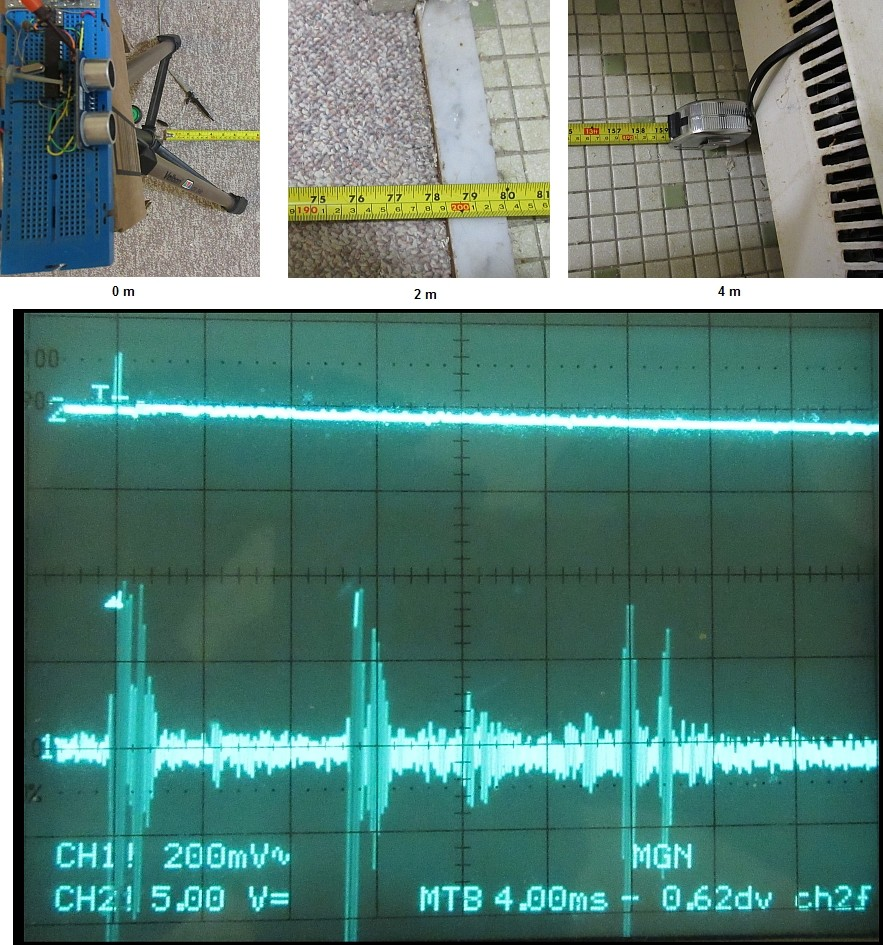
\includegraphics[max width=\linewidth]{pictures/had_us}
        \caption{Range profile measurement with a hacked HCSR04 ultrasound module. Source: \cite{Lee2015}}
        \label{fig:had_us}
    \end{subfigure}%
    \hfill%
    \begin{subfigure}[t]{0.56106798574\textwidth}
        \centering
        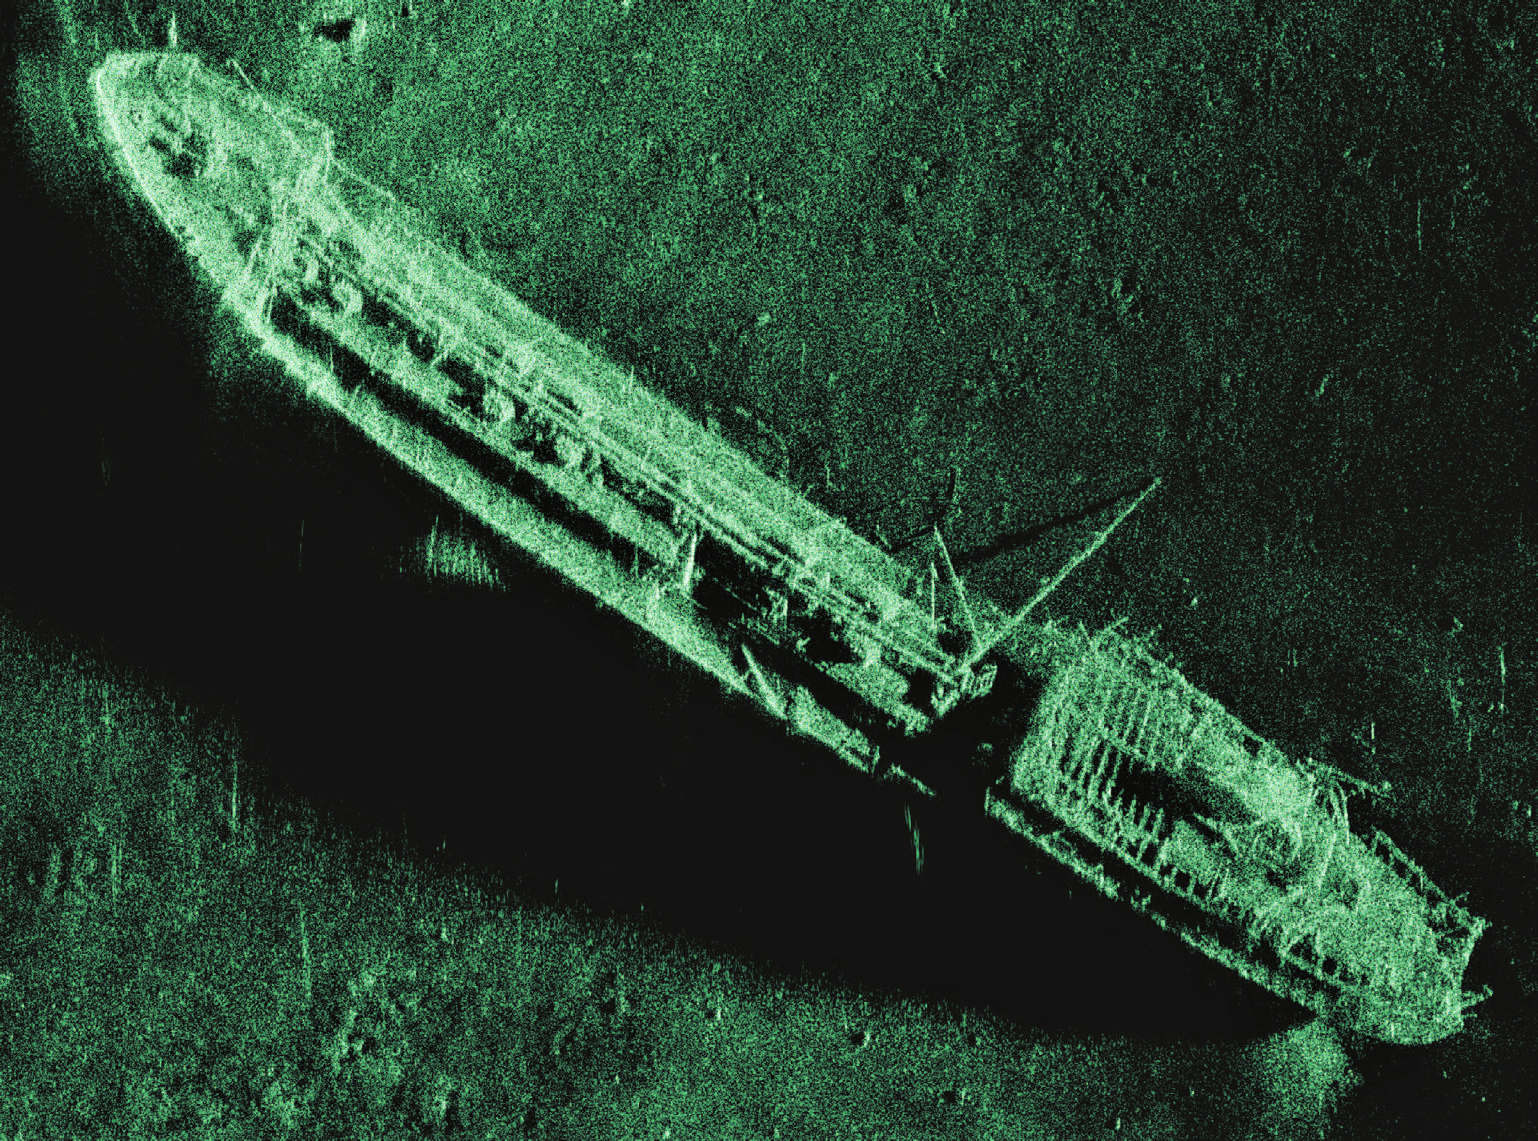
\includegraphics[max width=\linewidth]{gfx/pictures/sonar_sar}
        \caption{Synthetic aperture sonar imagery of a sunken ship. Source: \cite{Hansen2011}}
        \label{fig:sonar}
    \end{subfigure}
    \caption{Ultrasound might be a very interesting data source for reprojection mapping.}
    \label{fig:us}
\end{figure}

Most ultrasound range sensors use the time of flight of a pulsed echo,
but FMCW-based ultrasound modules have been proposed
\cite{Battaglini2014} recently. With a range resolution of
\begin{equation}
    dR = \frac{c_{sound, air}}{2 BW} = \frac{\SI{330}{m\per s}}{2\cdot \SI{12.5}{kHz}} = \SI{1.32}{cm}
\end{equation}
the proposed sensor would be comparable to the Omniradar sensor's range
resolution and accuracy. However, for measurements to be very accurate
the speed of sound in air must be known as it depends on humidity and
temperature \cite{Bohn1987}.

For forward-facing geometry DOA is necessary to resolve the sign of the
reprojection angle. Sound waves do not not carry phase information, but
with a transducer array, direction of arrival can still be estimated
\cite{Kunin2010}.

Extension to ultrasound sensors would be a very interesting topic for
further work. It might even be possible to use light waves with interferometric
modulated flash lidars and the right optics.

\section{Conclusion}\label{conclusion-1}

This thesis showed that mobile robots still struggle to detect some obstacles which are invisible to their conventional sensors. The fact that these are not special edge cases but very common objects like chair legs and windows highlights how important it is to improve mapping in these real-world environments. Radar sensing fills a gap in the design space by exposing these hidden obstacles. It is already a tried and tested technology and has been deployed in many diverse fields, including far-range military reconnaissance, speed limit enforcement, and weather forecasting for decades. However, with new advances in system integration, miniaturization, and cost optimization, ultra-wide bandwidth radar sensing becomes very interesting even for consumer-grade ground robots.

With reprojection mapping, this thesis proposes a novel method for scanless radar-based mapping that further reduces the barrier that kept radar sensors out of robots for so long by obviating the need to actively steer the radar beam via mechanical scanning or beamforming. The most limiting factor in the application is the need for a static environment to assert that any target can be localized through its Doppler speed. In practice this constraint is not too hard to meet because many indoor robots are designed to operate unsupervised in environments without moving objects, like an office at night or an apartment during working hours.

Even though the ideas behind reprojection mapping are not complex or require complicated math, this kind of scanless mapping has never been shown before. One can assume the reason to be that in high-performance, high-cost radar mapping applications it is easier to use more specifically designed expensive or complex scanning sensors. On the other end of the spectrum, low-cost and high-volume products could use cheaper and proven traditional sensors like laser scanners. Only the advent of cheaper and smaller radar range sensors allowed the expansion of robotic design space into the corner in which reprojection mapping becomes useful.

That reprojection mapping is useful, and moreover that it works as designed, is shown with a proof-of-concept implementation. With this implementation, several obstacle maps were created from the radar scans of the experiments for this thesis. The maps prove that some previously undetectable obstacles, like glass walls and office chair legs, can now be detected and mapped.

The next step on the way to a mobile indoor robot proficiently navigating real-world environments is the implementation of an online version of reprojection mapping. This will also show if the results need to be further improved with more advanced noise rejection.
